\documentclass{article}
\usepackage{amsmath}
\usepackage{amssymb}
\usepackage{graphicx}
\usepackage{hyperref}
\usepackage[version=4]{mhchem}


\begin{document}
In the diagram, \(A B=a+b \mathrm{~cm}\) is the diameter of semicircle \(O\). Circle \(Q\) has the radius of \(r\) and is inscribed in circle \(O\), and is tangent to \(A B\) at \(D\). Let \(A D=a\) and \(D B=b(a>b)\). Find \(r\) in terms of \(a\) and \(b\).\\
\centering
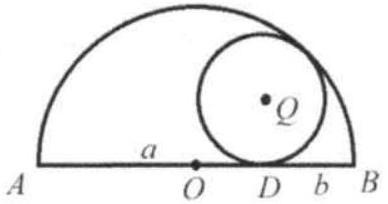
\includegraphics[width=\textwidth]{images/178(1).jpg}

Solution:
Connect \(O Q\) and extend it to meet the semicircle \(O\) at \(P\). Connect \(Q D\).

Since \(P\) is the tangent point of circle \(Q\) and semicircle \(O\),\\
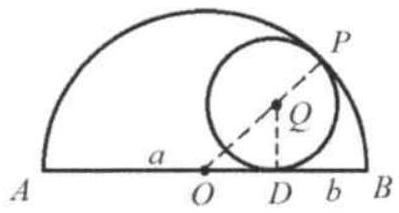
\includegraphics[width=\textwidth]{images/178(2).jpg} points \(O, Q, P\) are collinear.\\
\(O P=O A=O B=\frac{1}{2}(a+b)\)\\
\(O Q=O P-Q P=\frac{1}{2}(a+b)-r\)


\(O D=O D-D B=\frac{1}{2}(a-b)\).\\
In \(\triangle O D Q, O Q^{2}=Q D^{2}+O D^{2}\), or\\
\(\left[\frac{1}{2}(a+b)-r\right]^{2}=r^{2}+\left[\frac{1}{2}(a-b)\right]^{2}\).\\
Solving we get \(r=\frac{a b}{a+b}\) or \(\frac{1}{a}+\frac{1}{b}=\frac{1}{r}\).


\end{document}
